\documentclass{aicom2e}
\usepackage{amsmath}
\interdisplaylinepenalty=2500
\usepackage[algo2e,ruled,vlined,linesnumbered]{algorithm2e}
\usepackage[active]{srcltx}


\usepackage{amsthm, amssymb,amsfonts}
\usepackage{graphicx}
\usepackage{epsfig}
\usepackage{latexsym}
\usepackage{colortbl}
\usepackage{times}
\usepackage{helvet}
\usepackage{courier}
\usepackage{caption}
\usepackage{subfig}
\usepackage{float}
\usepackage{xcolor}
\usepackage{pslatex}
\usepackage{eso-pic}
\usepackage[bottom]{footmisc}
\usepackage{url}
\usepackage{etex}


\newtheorem{definition}{Definition}
\newtheorem{lemma}{Lemma}
\newtheorem{theorem}{Theorem}
\newcommand{\kgs}{$k$-goal search}
\newcommand{\kgbfs}{$k$-goal best-first search}


\newcommand{\astar}{A$^*$}
\newcommand{\tuple}[1]{\ensuremath{\left \langle #1 \right \rangle }}
\newcommand{\open}{\textsc{Open}}
%\newenvironment{proof}{\noindent{\bf Proof:~~}}{\qed}

\begin{document}
\begin{frontmatter}                           % The preamble begins here.
%
%\pretitle{Pretitle}
\title{Shortest Path for K Goals}
% \runningtitle{Running title}
%\subtitle{Subtitle}
\maketitle
%
\author[]{Meir Goldenberg}
\address{Lev Academic Center\\ Jerusalem, Israel\\
	E-mail: mgoldenbe@gmail.com}
\author[]{Roni Stern}
\address{Ben Gurion University of the Negev\\ Be'er Sheva, Israel\\
E-mail: roni.stern@gmail.com}
\author[]{Ariel Felner}
\address{Ben Gurion University of the Negev\\ Be'er Sheva, Israel\\
	E-mail: felner@bgu.ac.il}

\begin{abstract}
Abstract...

\end{abstract}

\begin{keyword}
artificial intelligence\sep AI\sep Heuristic Search
\end{keyword}
%
\end{frontmatter}

\section*{Introduction}


The shortest path problem (SSP) in a graph is the problem of finding the lowest cost path in a graph from one vertex -- denoted the {\em start} vertex -- to another vertex -- denoted the {\em goal} vertex. 
SSP is a well-studied problem and many algorithms have been proposed for solving it. 

Now, imaging $k$ SSP problems, such that all the problems share the same start vertex. 
Solving this set of SSP problems is called the $k$-goal problem. 
A trivial solution to \kgs\ is to run a SSP solver $k$ times. Alternatively, 
we can construct a $k$-dimensional SSP problem, and try to solve all the $k$ SSP problems concurrently. 
In this work we study the interplay between these two extreme approaches and
study how heuristics can be used correctly to solve \kgs. 

\section{Background and Problem Definition}

%In this section, we formally define the $k$-goal search problem.
In this section we provide relevant background and formally define the \kgs\ problem. 
Let $G=(V,E,w)$ be a weighted graph, where $w:E\rightarrow \mathbb{R}^+$ be the weight function, i.e., for an edge $e\in E$ the value $w(e)$ is its weight. 
The shortest path problem (SPP) is the problem of finding the lowest cost path in $G$ from a given start vertex $s$ to a goal vertex $g$. 

SPP has been well-studied in the literature. A popular framework for solving SPP is Best-first search (BFS). There are many path-finding algorithms that are based on BFS, including classical SPP algorithms like Dijkstra's algorithm~\cite{} and \astar{}. 
    While BFS has many variants, Algorithm~\ref{alg:bfs} provides a high-level pseudo-code for BFS. 


[[TODO: Background on BFS and on \astar{}. Talking also about admissible heuristics]]


\begin{algorithm2e}[t!]
	\KwIn{Start state $s$, Goal state $g$)}
    \open{}~$\gets\{s\}$; \\
    \While {\open{} $\neq \emptyset$} {
        $best \gets \texttt{ChooseNode}(\open{})$ \nllabel{line:open:chooseNode}\\
        Remove $best$ from \open{}\\
                \lIf {$best$ is a goal}{\Return $best$}
        \For{$n \in neighbors(best)$}{
            Add $n$ to \open{}\\
        }
    } 
\caption{Best-first-search}
\label{alg:bfs}
\end{algorithm2e}




The $\texttt{ChooseNode}$ function (line~\ref{line:open:chooseNode} in Alg.~\ref{alg:bfs}) is often implemented by defining a node evaluation function $F$, such that 
the chosen node is the one with the minimal $F$ value. For example, Dijsktra's algorithm is a BFS in which $F=g$, and \astar{} is a BFS in which $F=f=g+h$. 




The $k$-goal search problem can be viewed as a generalization of SPP, and is defined as follows. 

\begin{definition}[$k$-goal search]
Given a weighted graph $G$, a start vertex $s\in V$, and $k$ goal vertices 
$g_1, g_2,\ldots g_k\in V$, the task is to find $k$ paths $p_1,\ldots p_k$ 
such that for every $i\in [1,k]$ it holds that $p_i$ is a lowest-cost path from $s$ to $g_i$. 
\end{definition}

% k searches independentaly
Clearly, SPP is a special case of \kgs\ with $k=1$. A trivial solution to the \kgs\ problem is to consider it as $k$ independent shortest path problem, and use a SPP algorithm such as Dijkstra's algorithm~\cite{} or \astar{}~\cite{}. 
In this work we explore different approaches for solving the \kgs\ problem that try to reuse information between the $k$ tasks. 


\section{One BFS for $k$-Goal Search}

In this section we explore how to find solve the \kgs{} using a single BFS. This is motivated by the understanding that performing $k$ different searches may explore the same node multiple times. The main modifications done to the classical BFS are:
\begin{itemize}
    \item {\bf Stopping condition.} When one of the goal vertices is expanded, the found path to that goal is returned to the user. However, the search does not halt until lowest-cost paths to all $k$ are found. Therefore, after a path to a goal is found the search continues, expanding the found goal vertex and inserting its children to \open . The search only halts after there is a path found for every goal. 
    \item {\bf Tracking the relevant goals.} When searching for $k$ goals in a single BFS, we need to keep track of which goal has been solved, 
    i.e., a path to it has been found, and which goals still need to be found. 
    \item {\bf Node evaluation function.} When searching for a single lowest-cost path with \astar{}, the nodes are popped from \open{} 
    according to their $f=g+h$ values. To extend BFS to solve the \kgs\ problem efficiently, 
    we will associate nodes in \open{} with a value that considers the $h$-value for each of the $k$ goals. 
    Thus, when a node is generated then we compute the heuristic for each of the $k$ goals.
\end{itemize}



\begin{algorithm2e}[t!]
	\KwIn{Start state $s$, goal states $G_1,\ldots,G_k$}
	%\SetKwBlock{KGBFS}{$k$-goal best-first-search(start state $s$, goal states $G_1,\ldots,G_k$)}
	\open{}~$\gets\emptyset$ \\
	{\tt RelevantGoals} $\gets \{G_1,\ldots,G_k\}$ \nllabel{line:init-relevant-goals} \\
	$F_s\gets$ ComputeF(s, RelevantGoals) \nllabel{line:compute-f-start}\\
	Add $s$ to \open{} with key $F_s$ \\		
	\While {\open{} $\neq \emptyset$ and {\tt RelevantGoals} not empty} {
		$best \gets$ node in $\open{}$ with the smallest key \nllabel{line:open:chooseNode}\\
		Remove $best$ from \open{}\\
		\lIf {if $best\in$ {\tt RelevantGoals}}{
			Add path to $best$ to the solution \nllabel{line:storePath}\\
			Remove $best$ from {\tt RelevantGoals} \nllabel{line:removeGoal}\\
		}
		\For{$n \in neighbors(best)$}{
			$F_n\gets$ ComputeF(n, {\tt RelevantGoals})
			Add $n$ to \open{} with key $F_n$ \\
		}
	}
	\caption{\kgbfs{}}
	\label{alg:k-goal-bfs}
\end{algorithm2e}

Algorithm~\ref{alg:k-goal-bfs} shows the pseudo code for a BFS algorithm for solving the \kgs\ problem. 
Initially, all goals are inserted into the {\tt RelevantGoals} list (line~\ref{line:init-relevant-goals} in Alg.~\ref{alg:k-goal-bfs}), 
and the initial state is inserted into \open{} (line~\ref{line:compute-f-start}). 
Every node that is added to \open{} is associated with a key value 
that is computed using the {\tt ComputeF} function.  
Later in the paper we discuss how to implement this function. 
In every iteration, the node with the smallest key value is popped out of \open{} (line~\ref{line:open:chooseNode}). 
If it is a goal then we store the path to it (line~\ref{line:storePath}). In addition, we remove that goal from
the {\tt RelevantGoals} list, to mark that we are no longer looking for a path to that goal (line~\ref{line:removeGoal}). 
When the {\tt RelevantGoals} list is empty, we halt the search, having found a path to each goal. 


It is easy to see that Algorithm~\ref{alg:k-goal-bfs} is complete and sound, in the sense that if there are paths to the $k$-goals they will be found,
and the paths returned by the algorithm are all valid paths to the $k$ goals. The key question is whether these paths are indeed the optimal path to the $k$-goals.
As we show next, this depends on the order according to which nodes are expanded, 
which in turn depends on how the {\tt ComputeF} function is implemented. 

In regular \astar{} for a single goal, {\tt ComputeF} returns the $f=g+h$ value of a node. 
In \kgs{}, however, there are $k$ heuristic values for each node $n$, $h_1(n),\ldots,h_k(n)$,  where $h_i$ is the heuristic estimate of the cost to get from $n$ to goal $G_i$.  
Consequently, each node has multiple  $f$ values, $f_1(n),\ldots,f_k(n)$, one per goal. 
This raises the question of how to define the node evaluation function $F$ for \kgs{}, 
i.e,. which node to choose from \open{} in every iteration when solving the \kgs{} problem?


We discuss next the following two options. 
\begin{itemize}
 \item {\bf Min-$f$.} $F_{min}(n)=\min_{i\in [1,k]}f_i(n)$. 
 \item {\bf Max-$f$.} $F_{max}(n)=\max_{i\in [1,k]}f_i(n)$. 
 %\item {\bf Random-$f$.} $F(n)=ChooseRandom(f_1(n),\ldots,f_k(n))$. 
\end{itemize}

\subsection{$F_{min}$}

\begin{theorem}[Min-$f$ is admissible]
If $h$ is an admissible heuristic, then running Algorithm~\ref{alg:k-goal-bfs} with $F_{min}$ 
as the node evaluation function ({\tt ComputeF}) will return an optimal solution, i.e., 
it returns $k$ paths $\pi_1,\ldots, \pi_k$ such for every $i$ we have that $\pi_i$ is a lowest cost path from $s$ to $G_i$. 
\label{the:min-f}
\end{theorem}
 \begin{proof}
To prove this, we show that when a goal node is expanded for the first time, then its $g$ value is guaranteed to 
be the cost of the lowest-cost path from $s$ to that goal. 
By negation, assume that a goal $G_i$ was expanded, but there is a better path to $G_i$
that has not yet been discovered. Since the search is a best-first search, this means
that \open{} has some node $n$ that is on a better path to $G_i$ and has not been expanded yet. 
That is, 
\begin{equation}
g(n)+h_i(n)<g(G_i)
\label{eq:proof-1}
\end{equation}
Since $G_i$ was chosen to be expanded before $n$, it must have a $F_{min}$ value no-larger than $n$, i.e.,
\begin{align}
F_{min}(n) \geq & F_{min}(G_i)\\
g(n)+\min_j h_j(n) \geq & g(G_i)+\min_{j'} h_j(G_i)\\
g(n)+\min_j h_j(n) \geq & g(G_i)\\
g(n)+h_i(n) \geq & g(G_i) 
\end{align}
The last line above exactly contradicts Equation~\ref{eq:proof-1}. 
\end{proof}



\subsection{$F_{max}$}
 
 \begin{figure}
 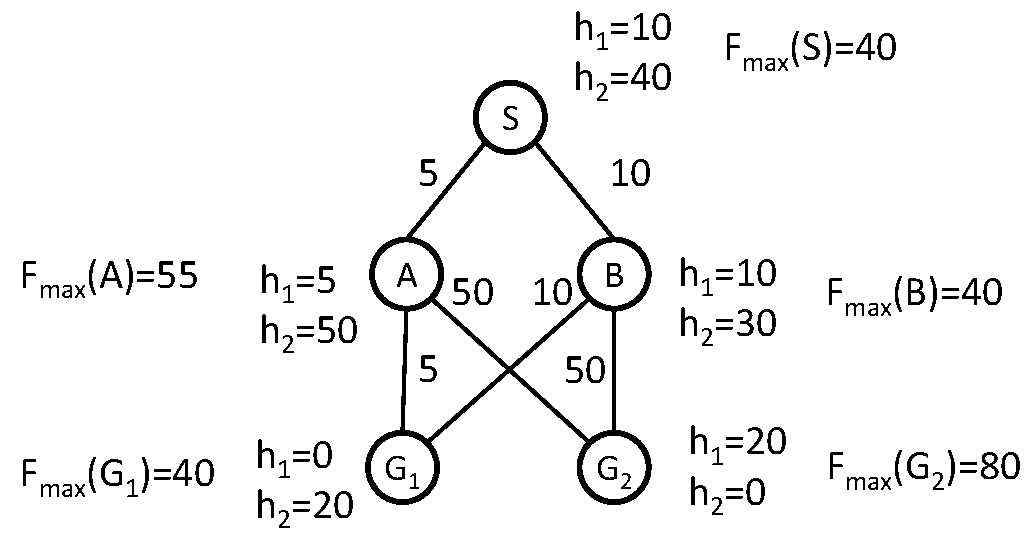
\includegraphics[width=\columnwidth]{max-bad_cropped.pdf}      
 \caption{An example of where using Max-$f$ returns a non-optimal solution. In this example, 
 using Max-$f$ will results in the following expansion order: $S$, $B$, $G_1$. 
 Thus, when $G_1$ is expanded, the best path known to it costs 25, while a 
 better path to it goes through $A$ and costs only 10.}
 \label{fig:max-bad}
 \end{figure}
 
 When using Max-$f$, however, expanding a goal $g_i$ does not guarantee
 that the optimal solution to $g_i$ has been found. As a counter-example, consider 
 the graph in Figure~\ref{fig:max-bad}.
 In this example, using Max-$f$ will result in the following expansion order: $S$, $B$, and then $G_1$. At this stage, we expanded one of the goals -- $G_1$ -- while the best path found so far to it goes through $B$ and costs 40. However, a better path to it is through $A$, which costs only 10.
 
 
 Of course, one may still use Max-$f$ as an anytime algorithm. 
 Instead of assuming that when expanding a goal the best path to it has been found, we continue the search, , still looking for better path to that goal. The search halted when 
 [[Roni: do we still need to compute the heuristic for these goals?]]
 [[Roni: What is a good stopping condition for this option?]]
 %Concretely, we continued to compute the heuristic for all goals even after they were expanded, thus continuing to guide the search to look for better path continuing the search and looking for better path to the previously expanded goals. 
 
 \subsubsection{Max-$f$ and Consistency}
 Interestingly, the inadmissibility of Max-$f$ is related to the {\em inconsistency} of the used heuristic. 
  \begin{definition}[Inconsistent Heuristic]
 A heuristic $h$ is inconsistent if there exists a pair of states $x$ and $y$ such that
 \[ h(x)>c(x,y)+h(y) \]
 where $c(n,c)$ is the least cost path from $x$ to $y$
 \label{def:inconsistent}
 \end{definition}
 The observant reader may have noticed that the heuristic function in the example in Figure~\ref{fig:max-bad} is indeed inconsistent: $h_2(A)=50$ while its child, $G_1$, which is connected to it via an edge of cost 5, has $h_2(G_1)=20$. If $h$ was consistent the $h_2(A)-c(A,G_1)\leq h_2(G_1)$, where e$c(A,G_1)$ is the cost of the edge between $A$ and $G_1$. 
 
 
\begin{theorem}[Max-$f$ is admissible if $h$ is consistent]
If $G$ is undirected and $h$ is admissible and consistent, 
then when running \kgbfs{} that uses Max-$f$ as an evaluation function,
it holds that whenever a goal is expanded then the lowest-cost path to it has been found. 
\label{the:max-f}
\end{theorem}
 \begin{proof}
 Assume by negation that Theorem~\ref{the:max-f} is not correct. This means
 that there is a case where a goal $G_i$ is expanded while $g(G_i)$ is not optimal. Since we are running a BFS, this means that there exists a node $n\in OPEN$ that is on the optimal path to $G_i$ and for which $g(n)=g^*(n)$. Formally, 
 \begin{equation}
     g(n)+h_i^*(n) = g^*(n)+h_i^*(n) < g(G_i)
    \label{eq:not-optimal}
 \end{equation}
 
 Now, since $G_i$ was chosen for expansion and not $n$, it holds that $F_{max}(n)  > F_{max}(G_i)$. Following the definition of $F_{max}$, we have that
 \begin{equation}
     g(n)+\max_j h_j(n) > g(G_i) + \max_{j'} h_{j'}(G_i)
 \end{equation}
 So, there exists a goal $G_l$ for which $f_l(n)$ is larger than 
 all the $f_j$ values of $G_j$, for every $j\in [1,k]$. In particular, 
 $f_l(n)>f_l(G_i)$, and consequently:
 \begin{align}
     g(G_i)+h_l(G_i) < & g(n)+h_l(n) \\
     g(G_i) < & g(n)+h_l(n) - h_l(G_i) 
 \end{align} 
Now, since we assumed that we have not found the optimal path to $G_i$ (Eq.~ \ref{eq:not-optimal}) then:
\begin{align}
\Rightarrow g(n)+h^*_i(n)  & < g(n)+h_l(n) - h_l(G_i)\\
\Rightarrow h^*_i(n)  & < h_l(n) - h_l(G_i)\\
\Rightarrow c(n,G_i) + h_l(G_i) & < h_l(n) \label{eq:h-inconsistent} 
\end{align}
Thus, Equation~\ref{eq:h-inconsistent} directly contradicts the assumption
that $h$ is consistent (see Definition~\ref{def:inconsistent}). 
\end{proof} 


\section{Runtime Analysis}
% Analysis
Now, we compare the the two approaches descibed bove -- $k$ separate SPP problems or one BFS to return all the $k$ paths. 
It is common to estimate the runtime of BFS by counting the number of nodes that are expanded until the goal is found. However, we can show that both approaches will expand the same set of nodes.  However, the computation done per node is different. 

[[Here will come Ariel's analysis of the runtime]]

\subsection{Optimally Effective}
One of the well-known properties of \astar{} is that it is {\em optimally effective}~\cite{dechter}. Informally, this means that given an admissible heuristic $h$, \astar{} will expand no more nodes than any other best-first search
that uses the same heuristic function, up to tie breaking. 
A more recent generalization of \astar{} also provides a similar guarantee
with respect to the number of nodes generated~\cite{Goldenberg}. 
In this section we ask whether we can say something similar about the proposed
best-first search for \kgs{}. 

\begin{definition}[Surplus Nodes and Necessary nodes]
A node $n$ is called a surplus node if $g(n)+h(n)>opt$, where $opt$ is the cost of the lowest cost path. 
A node $n$ is called a necessary node if $g(n)+h(n)<opt$, where $opt$ is the cost of the lowest cost path. 
In the contest of the \kgs{} problem, we say that a node $n$ is a surlpus node for goal $G_i$ if $g(n)+h_i(n)>opt_i$, where $opt_i$ is the cost of hte lowest cost path to $G_i$ (from the initial state). Similarly, $n$ is a necessary node for $G_i$
if $g(n)+h_i(n)<opt_i$. 
\end{definition}
It is know that an \astar{} search using $h_i$ 
must expand all necessary nodes and will not expand any surplus node. 


\begin{lemma}
\kgbfs{} with the Min-$f$ evaluation function never expands a node
that is a surplus node for all goals. 
\label{lem:min-f-no-surplus}
\end{lemma}
The consequene of Lemma~\ref{lem:min-f-no-surplus} is 
that \kgbfs{} with the Min-$f$ evaluation function expands no more nodes
than running $k$ \astar{} searches, up to tie breaking. This suggests towards the 
effectiveness of $kgbfs{}$. Interestingly, this property does not hold when using
the Max-$f$ evaluation function. To show this, consider a \kgs{} problem with two goals 
$G_1$ and $G_2$ (i.e., $k=2$). Now, assume that $opt_1=opt_2=2$
and that the open list has three nodes $n_1, n_2,$ and $n_3$, such that
their $g$ values is one, and the $h_1$ values of $n_1, n_2,$ and $n_3$
are $9,5,$ and $1$, respectively, and the $h_2$ values of $n_1, n_2,$ and $n_3$ 
are $1,5,$ and $9$ respectively. Consequently, the $f$ value for $n_1, n_2,$ and $n_3$
when using Max-$f$ are $10,6,$ and $10$, respectively. Thus, node $n_2$ will be expanded
while it is a surplus node for $G_1$ and for $G_2$. 





\section{Experimental Results}
[[Here will come experimental results]]

\subsection*{Related work}

There are several well-studied graph problems that are related to $k$-goal search. In the traveling salesman problem (TSP), we aim to find a shortest path that passes through a set of vertices. 
...

\section{Conclusion and Future Work}

% \begin{figure}[!htbp]
%   \centering
%   \includegraphics[width=1\hsize]{filename.eps}
%   \caption{caption} \label{fig:label}
% \end{figure}

\section*{Acknowledgements}
Thanks!

\bibliographystyle{abbrv}
\bibliography{library}

\end{document}
